% !TeX TS-program = xelatex

\documentclass{resume}
\usepackage{graphicx}
\usepackage{tikz}
\ResumeName{周信航}

\begin{document}

% 照片绝对定位到页面右上角，不占用正文排版空间
\begin{tikzpicture}[remember picture, overlay]
  \node[anchor=north east, inner sep=0pt, xshift=-1.2cm, yshift=-1cm]
    at (current page.north east)
    {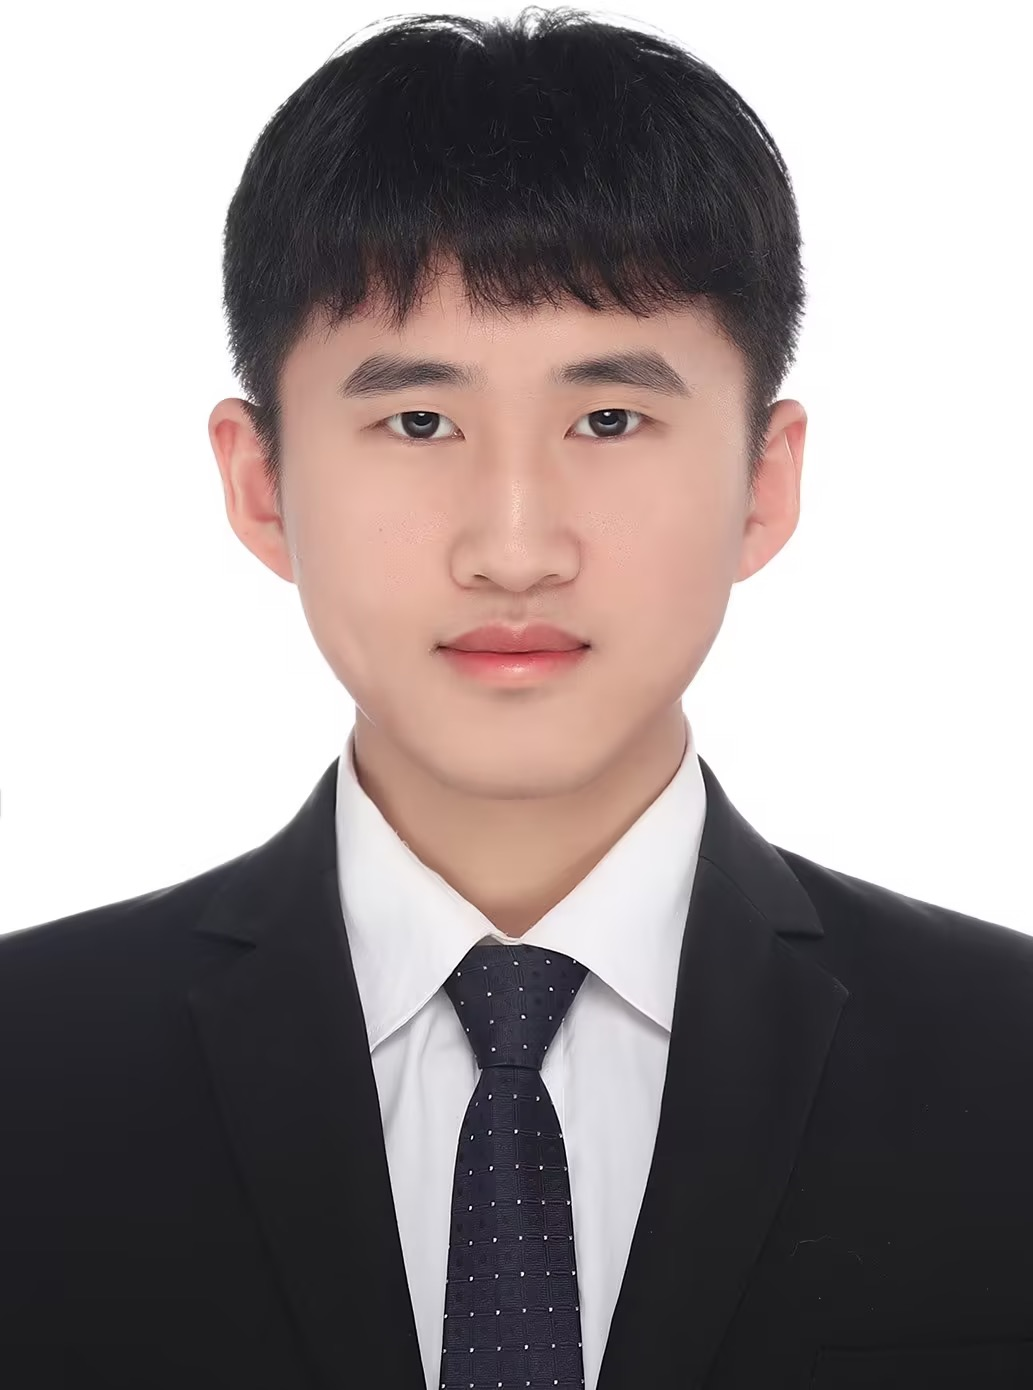
\includegraphics[height=3.4cm, keepaspectratio=true]{main.jpg}};
\end{tikzpicture}

\ResumeContacts{
  (+86)13382788320,%
  \ResumeUrl{mailto:xxx@example.com}{zxhccp@163.com}%
}

\ResumeTitle

\vspace{1em}

\section{教育经历}
\ResumeItem
[大连理工大学|硕士研究生]
{大连理工大学}
[\textnormal{车辆工程专业，机械学院|}  硕士研究生]
[2022.09—2025.06]

% TODO: 补充GPA、研究方向、论文等信息

\ResumeItem
[南京工业大学|本科生]
{南京工业大学}
[\textnormal{车辆工程专业，机械学院|} 工学学士]
[2018.09—2022.06]

% TODO: 补充GPA、奖项等信息

\section{技术能力}
\begin{itemize}
  \item \textbf{深度学习框架}: Python、PyTorch、PyTorch Lightning、HuggingFace Transformers、Hydra
  \item \textbf{大模型与推理}: Qwen3-VL/Qwen3.5、vLLM、FlashAttention、M-RoPE、KV Cache
  \item \textbf{训练基础设施}: DDP、bf16 混合精度、WebDataset、Ray、MLflow、Git
  \item \textbf{研究方向}: 视觉-语言-动作（VLA）模型、自动驾驶端到端轨迹规划、多模态轨迹预测、世界模型、强化微调（GRPO）
\end{itemize}

\section{工作经历}

\ResumeItem{上海临港绝影智能科技有限公司}
[算法工程师 / VLA 方向] % TODO: 如职位有出入请修改
[2025.6—至今] % TODO: 补充入职时间

\begin{itemize}
  \item 参与自动驾驶 VLA（Vision-Language-Action）模型的预研与落地，覆盖从 VLM backbone 适配、轨迹规划 head 设计、训练框架搭建到典型场景效果验证的完整链路。
  \item 推动多个关键能力上车前实验：单模态 / 多模态轨迹规划、指令变道、施工绕行、OCC 世界模型辅助、GRPO 强化微调等。
\end{itemize}

\section{项目经历}

\ResumeItem{自动驾驶 VLA 端到端轨迹规划}
[核心研发] % TODO: 如有团队规模/职责描述可替换
[2025.06—至今]

\begin{itemize}
  \item \textbf{VLM 部署与场景理解评测}：基于 vLLM 部署 Qwen3-VL-8B-Instruct，构建典型驾驶场景测试集，评测模型对场景的理解能力、应采取动作的判断及完整推理链路输出。
  \item \textbf{单模态轨迹规划 backbone}：以 Qwen3-VL 为骨干，前视双相机图像以 Image Encoding 与 Video Temporal Encoding 两种方案接入；自定义 \texttt{<|nav\_i|>} / \texttt{<|plan\_q\_i|>} 占位 token 注入导航路径与 plan query；解码侧采用可微分 unicycle action rollout，head 直出 \texttt{(accel, yaw\_rate)} 经积分得到 50 步轨迹。Video Temporal Encoding 方案相对历史 Image 方案训练吞吐提升 1.47×，\textbf{ADE 降低 15.3\%、FDE 降低 18.3\%}。
  \item \textbf{训练性能优化}：通过 sequence packing + \texttt{flash\_attn\_varlen\_func} 变长注意力替换 Qwen3-VL 默认实现，配合 cu\_seqlens 边界传递与 3D 位置编码自定义计算，显著降低 padding 浪费、提升单卡吞吐。
  \item \textbf{OCC 世界模型辅助任务}：设计稠密 BEV 占用栅格世界模型 head（Geometry PE：ego 坐标 + 多相机投影 UV 联合编码、4 层 cross-attention、200×120 BEV 网格），并通过 BEV→plan query 的 cross-attention fusion 将占用特征反哺规划。在相同训练 step 下 \textbf{ADE 提升 10\%、FDE 提升 13\%、miss rate 降低 14\%}。
  \item \textbf{指令变道实验}：将 human command 文本注入 VLM 输入，通过在直行巡航场景注入 fake 变道指令验证模型响应能力，\textbf{fake 变道响应率接近 100\%}；同时模型能识别"最左侧车道无变道空间""路边停有死车"等场景并合理拒绝执行，证明模型具备一定的安全约束理解能力。
  \item \textbf{轻量化 backbone 探索（Qwen3.5-0.8B）}：针对车端推理资源受限的问题，将 VLA backbone 由 Qwen3-VL-2B 替换为 Qwen3.5-0.8B。轨迹任务指标对齐 2B 效果，叠加 OCC 辅助任务后略有提升；Torch 推理耗时降低 4 倍，成功支持 10 Hz 车端在线推理。
  \item \textbf{多模态轨迹规划}：基于 K-Means 聚类构建 64 锚轨迹库，head 输出 anchor 分类 + 残差回归，top1 指标略优于单模态；在汇入主路、进入辅路、施工绕行、跟车减速刹停等长尾场景输出高质量多模态轨迹。
  \item \textbf{GRPO 强化微调框架}：从 0 搭建基于 GRPO（Group Relative Policy Optimization）的 VLA 强化微调 codebase，为后续轨迹质量奖励 / 安全奖励等多奖励信号下的策略优化提供基础设施。
\end{itemize}

\section{个人总结}

\begin{itemize}
  \item 具备从 VLM 适配、训练加速、Head 架构设计到指标验证的端到端落地能力，熟悉 Qwen3-VL、3.5等系列模型内部机制（M-RoPE、视觉 patch 化、packing 注意力）。
  \item 关注训练效率与工程化质量，主动推进 packing/flash-attention/混合精度等基础设施优化以缩短迭代周期。
  \item 持续跟进 VLA、世界模型、强化微调等前沿方向，乐于把论文方法快速转化为可复现的实验代码。
\end{itemize}


\end{document}